\documentclass[a4paper]{article}

\usepackage{amsmath}
\usepackage{amssymb,amsfonts}
\usepackage[catalan]{babel} % Language 
\usepackage{fontspec} 
\usepackage[margin=2cm]{geometry}
\usepackage{graphicx}
\usepackage[makeroom]{cancel}
\usepackage{listings}
\usepackage[dvipsnames]{xcolor}
	
\usepackage{float}
\usepackage{xcolor}
\usepackage{listings}

\usepackage{xparse}
\setlength{\parindent}{0pt}
\setlength{\parskip}{0.2cm}

\usepackage{color}
\lstset{ %
	language=R,                     % the language of the code
	basicstyle=\footnotesize,       % the size of the fonts that are used for the code
	numbers=left,                   % where to put the line-numbers
	numberstyle=\tiny\color{gray},  % the style that is used for the line-numbers
	stepnumber=1,                   % the step between two line-numbers. If it's 1, each line
	% will be numbered
	numbersep=5pt,                  % how far the line-numbers are from the code
	backgroundcolor=\color{white},  % choose the background color. You must add \usepackage{color}
	showspaces=false,               % show spaces adding particular underscores
	showstringspaces=false,         % underline spaces within strings
	showtabs=false,                 % show tabs within strings adding particular underscores
	frame=single,                   % adds a frame around the code
	rulecolor=\color{black},        % if not set, the frame-color may be changed on line-breaks within not-black text (e.g. commens (green here))
	tabsize=2,                      % sets default tabsize to 2 spaces
	captionpos=b,                   % sets the caption-position to bottom
	breaklines=true,                % sets automatic line breaking
	breakatwhitespace=false,        % sets if automatic breaks should only happen at whitespace
	title=\lstname,                 % show the filename of files included with \lstinputlisting;
	% also try caption instead of title
	keywordstyle=\color{blue},      % keyword style
	commentstyle=\color{dkgreen},   % comment style
	stringstyle=\color{mauve},      % string literal style
	escapeinside={\%*}{*)},         % if you want to add a comment within your code
	morekeywords={*,...},
	          % if you want to add more keywords to the set
	alsoletter={.}        % if you want to add more keywords to the set
} 

\graphicspath{{images/}}
\title{Problemes APA \\ Problema 12: Clustering de les dades artificials de Cassini}
\author{Lluc Bové}
\date{Q1 2016-17}

\begin{document}

\maketitle

Volem analitzar un problema d'agrupament amb dades en 2D usant la rutina \lstinline{mlbench.cassini}. Generem dades en 3 grups amb el codi:\\

\begin{lstlisting}[frame=none,numbers=none]
	library(mlbench)
	
	N <- 2000
	
	data.1 <- mlbench.cassini(N, relsize = c(1,1,0.25))
	
	plot(data.1)
\end{lstlisting}
 
 Veiem que les estructures externes tenen forma de plàtan i entre elles hi ha un cercle amb menys densitat de dades. El \lstinline|plot| anterior mostr la veritat de les dades (els $3$ grups generats). Si ara fem:
 
 \begin{lstlisting}[frame=none,numbers=none]
plot(x=data.1$x[,1], y=data.1$x[,2])
 \end{lstlisting}
 
 Veurem les dades en brut (el que rebrà el mètode de \textit{clustering}). Es demana:
 
 \begin{enumerate}
 	\item \textbf{ Decidiu per endavant quin mètode de \textit{clustering} hauria de treballar millor i amb quins paràmetres} \\
 	El millor mètode hauria de ser barreja de gaussianes, donat que k-means aquí no tindria resultat, ja que a simple vista es pot veure que no seria el cas de gaussianes esfèriques. Pel que fa la família de la gaussiana en qüestió, sabent com s'han generat les gaussianes podríem elegir usar la família diagonal ja que les variables són independents. Però com que assumim que no sabem la veritat sobre les dades usarem general com a família de gaussianes.

 	\item \textbf{Apliqueu k-means un cert nombre de vegades amb $k = 3$ i observeu els reultats}\\
 	Al aplicar k-means un cert nombre de vegades i quedant-nos amb la millor execució basant-nos en l'índex de \textit{Calinski-Harabasz } amb $k = 3$ ens trobem amb la següent partició:
	 
	\begin{figure}[H]
	\centering
 	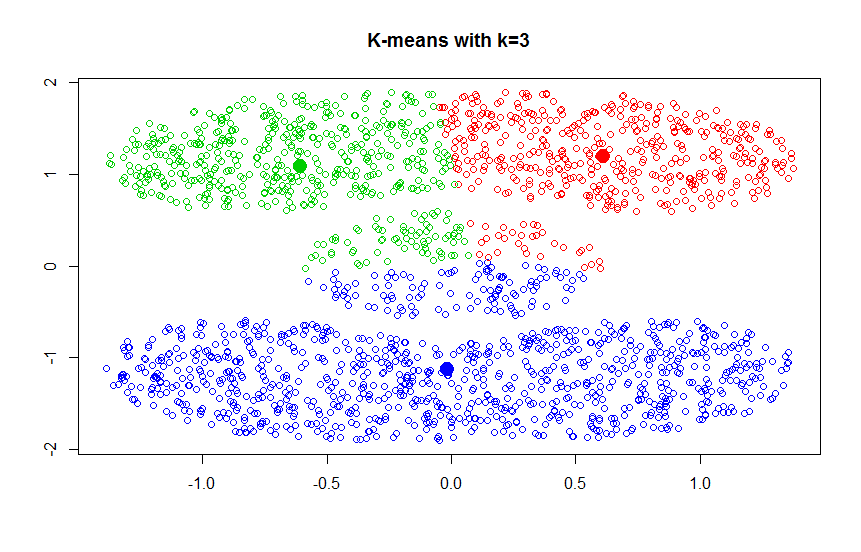
\includegraphics[scale=0.5]{3kmeans}
	\end{figure}
 	Podem veure que no s'acosta gens a la partició original, el \textit{cluster} circular original fa que formi part de tots els \textit{clusters} nous. El resultat és l'esperat ja que les dades no estan generades per gaussianes esfèriques i per tant k-means no ajusta massa bé.
 	
 	\item \textbf{Apliqueu k-means amb una selecció de valors de k al vostre criteri (20 cops cadascun) i monitoritzeu l'índex de Calinski-Harabasz mitjà; quin k es veu millor?} \\
    Usem valors de $k$ en l'interval $[2,10]$ i executem 20 cops per cada valor de $k$, trobem que la millor $k$ varia depenent de l'execució general, entre els valors $2$ i $5$. En aquest cas mostrem el gràfic d'evolució de l'index CH segons el valor de $k$, en que el cas millor és $k = 2$:
    
    	\begin{figure}[H]
    	\centering
    	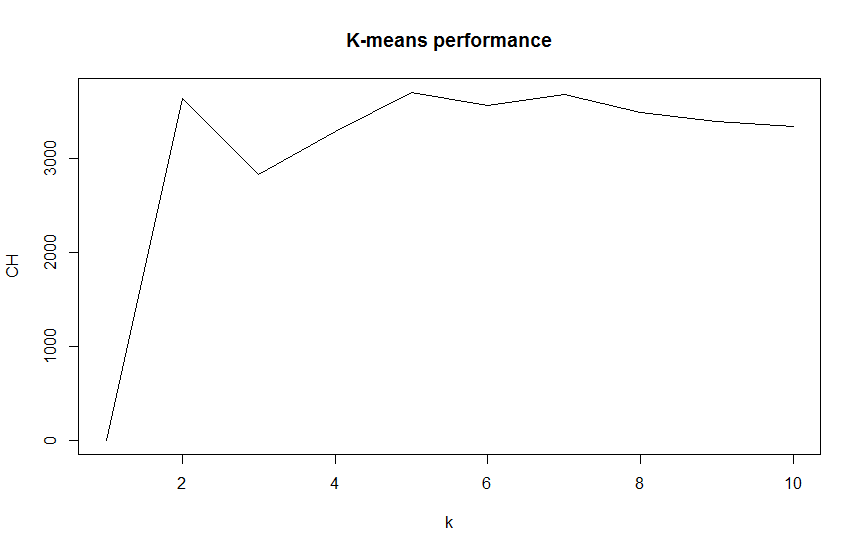
\includegraphics[scale=0.5]{kmeansPerf}
	    \end{figure}
    
    Veiem doncs que els valors més alts de $k$ són 2 i 5, i el més alt entre ells dos és 2. Mostrem doncs el \textit{clustering} amb $k = 2$.
    
    \begin{figure}[H]
    	\centering
    	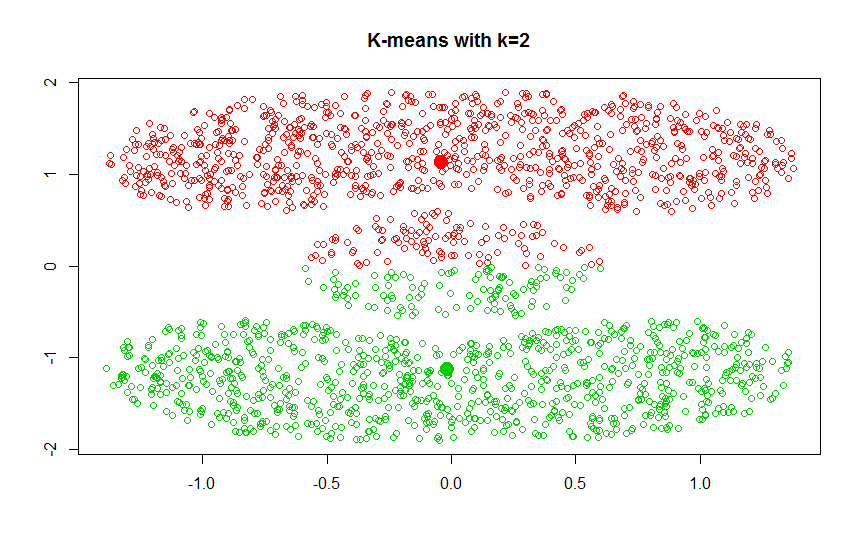
\includegraphics[scale=0.5]{2kmeans}
    \end{figure}

 	Segurament aquesta partició tingui un millor índex ja que es redueix la variància entre els \textit{clusters} i també la variància dins d'ells. Tot i això no és el que busquem, com es pot veure a simple vista, ja que ni tant sols la millor $k$ coincideix amb el nombre real de classes.
 	
 	\item \textbf{Apliqueu l'algorisme E-M amb una selecció de valors de k al vostre criteri (10 cops cadascun) i observeu els resultats. Comproveu els resultats contra les vostres expectatives (apartat 1).}\\
 	Apliquem E-M per valors de $k$ dins de l'interval $[2-5]$. Primer provem de mesurar l'índex CH per a tots els valors de $k$ i obtenim el següent gràfic:
 	
 	\begin{figure}[H]
 		\centering
 		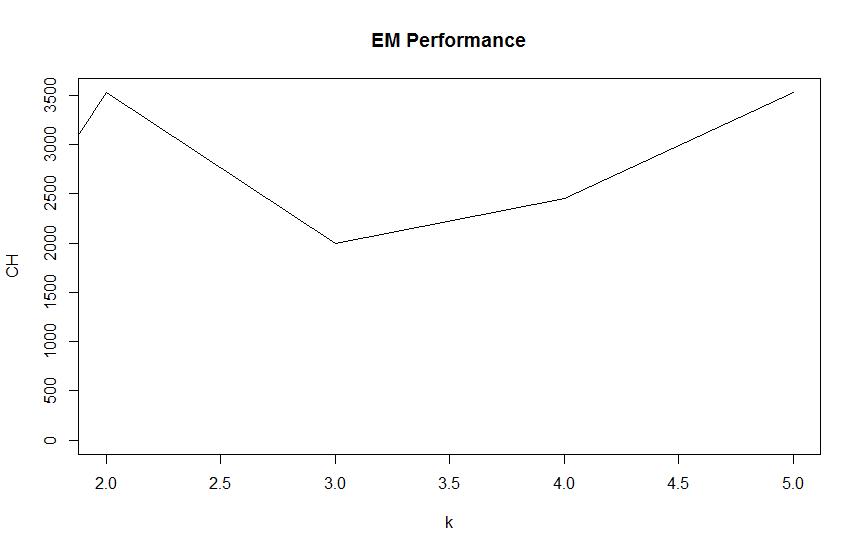
\includegraphics[scale=0.5]{CHPerf}
 	\end{figure}
 
   Podem veure com el millor valor de k és $5$. Això contradiu el que esperàvem ja que sabem que el nombre de \textit{clusters} és 3 i justament amb $k=3$ tenim el valor més baix de l'index mesurat. A més a més hauria d'ajustar millor amb els paràmetres de EM que hem elegit. Així doncs pensem que l'índex CH potser no és el més adequat per mesurar la qualitat de la partició de les nostres dades i per això provem el mateix experiment amb l'índex BIC(\textit{Bayesian information criterion}). Aquest índex es basa en la versemblança de la partició i com més baix és, més bona és aquesta. Obtenim el següent:
   
    \begin{figure}[H]
   	\centering
   	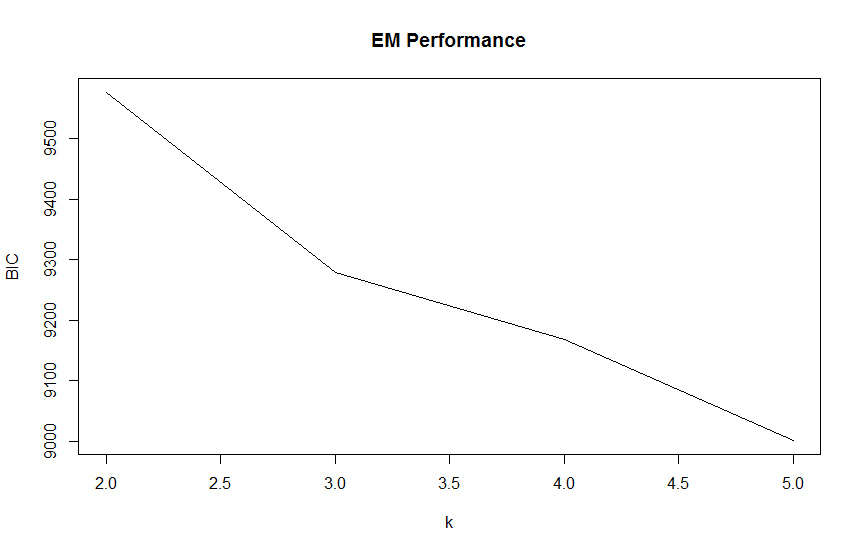
\includegraphics[scale=0.5]{BICPerf}
   \end{figure}

 Podem veure com tampoc és gaire bo l'índex pel que fa la decisió de $k$ ja que al augmentar-la aquest disminueix. Per tant la millor $k$ tampoc seria 3 com ja sabem que ha de ser. Així doncs creem un nou criteri per a trobar la qualitat de la partició, ens basem en la veritat de les dades. Aquest criteri no és realista ja que normalment no saps la partició a priori de les dades, però com que estem analitzant el comportament dels algorismes de \textit{clustering} farem veure que sabem a priori com és la partició. Així doncs anomenem aquest criteri \textit{diff} i expressa quants punts no "encaixen" en la partició vertadera. És a dir, actuaria com una diferència entre la partició original i la que trobem amb l'algorisme. Mesurem també l'index per a la selecció de $k$ i ho representem:
 
  	\begin{figure}[H]
 	\centering
 	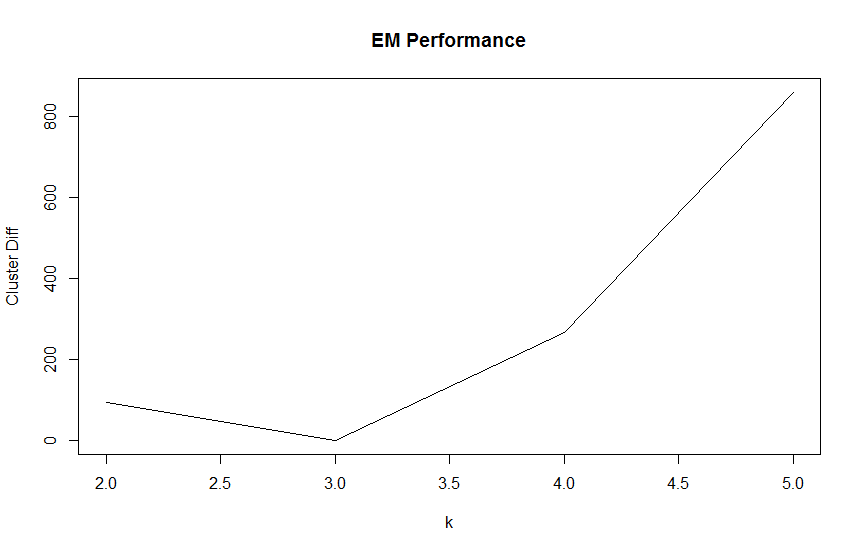
\includegraphics[scale=0.5]{DifPerf}
 \end{figure}

Aquí sí que es veu clarament com el millor valor de $k$ és 3. Sabent això executem unes quantes vegades l'algorisme EM amb $k=3$ i ens quedem amb la millor execució i podem observar el \textit{clustering} que veiem a continuació:

 	\begin{figure}[H]
	\centering
	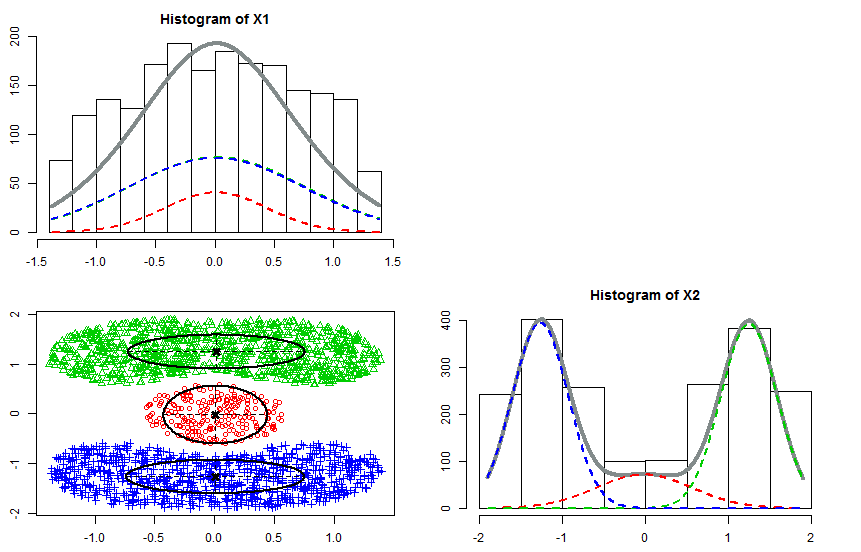
\includegraphics[scale=0.5]{diffResult}
	\end{figure}
 
Amb un bon nombre d'execucions hem pogut obtenir un \textit{clustering} que és igual al vertader, és a dir, s'ajusta a la perfecció. Amb tot això podem dir que si no tenim dades a priori sobre el nombre de \textit{clusters} que hem d'obtenir és molt complicat trobar un criteri que avaluï una partició concreta per poder optimitzar aquest nombre, i per tant, trobar quants \textit{clusters} hem de buscar i que a més a més sigui independent de com són les dades.
 \end{enumerate}




\end{document}